\section{Resultados Experimentais}
\label{sec:resultados_experimentais}

A validação experimental do sistema de navegação autônoma desenvolvido para a plataforma VIDA foi realizada por meio de ensaios em ambiente real, buscando avaliar a integração dos subsistemas de sensoriamento, estimação de estados, controle de baixo nível e seguimento de trajetórias. Os experimentos permitiram verificar o funcionamento da arquitetura computacional distribuída e avaliar o comportamento do veículo durante a execução autônoma de percursos previamente definidos.

Foram realizados dois experimentos de seguimento autônomo de trajetória, denominados Trajeto 1 e Trajeto 2. A avaliação foi conduzida a partir dos dados registrados pelo ROS~2, considerando as trajetórias de referência e executadas, os erros de seguimento, os comandos de controle e as informações disponibilizadas pelo estimador de estados.

\subsection{Procedimento Experimental}
\label{subsec:procedimento_experimental}

Os ensaios foram realizados com a plataforma VIDA, utilizando os subsistemas de controle, localização e navegação apresentados nas seções anteriores.

As trajetórias de referência foram obtidas a partir de coordenadas geográficas registradas pelo receptor GNSS durante a condução manual do veículo. Os pontos coletados foram posteriormente processados por meio de suavização e reamostragem, resultando em trajetórias com espaçamento uniforme de 0,25~m, armazenadas em arquivos CSV e utilizadas pelo sistema de navegação autônoma.

A preparação e o acompanhamento dos experimentos foram realizados com o auxílio do painel de operação e monitoramento apresentado na Seção~\ref{subsec:painel_operacao}. Por meio dessa interface, foi possível selecionar as trajetórias de referência, gerenciar a inicialização dos programas de navegação e acompanhar, em tempo real, as condições de segurança, localização e controle do veículo ao longo da execução dos percursos.

O desempenho dos controladores de baixo nível foi avaliado por meio da comparação entre as referências de velocidade longitudinal e ângulo de esterçamento e as respectivas respostas medidas durante os ensaios.

Em ambos os experimentos, foi utilizada uma referência de velocidade longitudinal de 2,0~m/s. Para a avaliação quantitativa do desempenho do seguimento, foram considerados o erro médio absoluto (MAE), a raiz do erro quadrático médio (RMSE) e o erro máximo absoluto, calculados a partir dos erros laterais registrados no decorrer da navegação autônoma:

\begin{equation}
    \mathrm{MAE} = \frac{1}{N}\sum_{i=1}^{N}|e_i|,
    \label{eq:mae}
\end{equation}

\begin{equation}
    \mathrm{RMSE} = \sqrt{\frac{1}{N}\sum_{i=1}^{N}e_i^2},
    \label{eq:rmse}
\end{equation}

\begin{equation}
    e_{\mathrm{max}} = \max_{1 \leq i \leq N}|e_i|,
    \label{eq:erro_maximo}
\end{equation}

em que $e_i$ representa o erro lateral registrado em cada amostra e $N$ corresponde ao número total de amostras consideradas. O erro máximo absoluto corresponde ao maior valor de $|e_i|$ observado durante cada experimento.


\subsection{Desempenho dos Controladores de Baixo Nível}
\label{subsec:resultados_baixo_nivel}

Os controladores de baixo nível desempenham um papel fundamental na execução dos comandos de navegação, sendo responsáveis por regular o ângulo de esterçamento e a velocidade longitudinal do veículo. Sua avaliação experimental busca verificar a capacidade de acompanhar as referências estabelecidas, bem como identificar possíveis limitações associadas à dinâmica dos atuadores. Os resultados são apresentados a seguir, iniciando pela malha de esterçamento e, posteriormente, pela malha de velocidade longitudinal.

O controlador PID de esterçamento apresentou capacidade de acompanhar as referências angulares fornecidas pelo controlador Stanley durante o seguimento autônomo de trajetória. Conforme apresentado na Figura~\ref{fig:resposta_esterçamento}, o ângulo medido pelo sensor LVDT acompanhou as variações da referência, apresentando RMSE de 1,68$^\circ$ e atraso estimado de aproximadamente 175~ms. Esse atraso pode estar associado à combinação de fatores como a filtragem do sinal do LVDT, a latência da comunicação entre os dispositivos, o atrito do mecanismo de direção e a zona morta do controlador. O erro máximo absoluto registrado foi de 4,47$^\circ$, observado após uma curva mais fechada à direita, quando a referência de esterçamento variou rapidamente de aproximadamente 20$^\circ$ para $-20^\circ$.

\begin{figure}[htb]
    \centering
    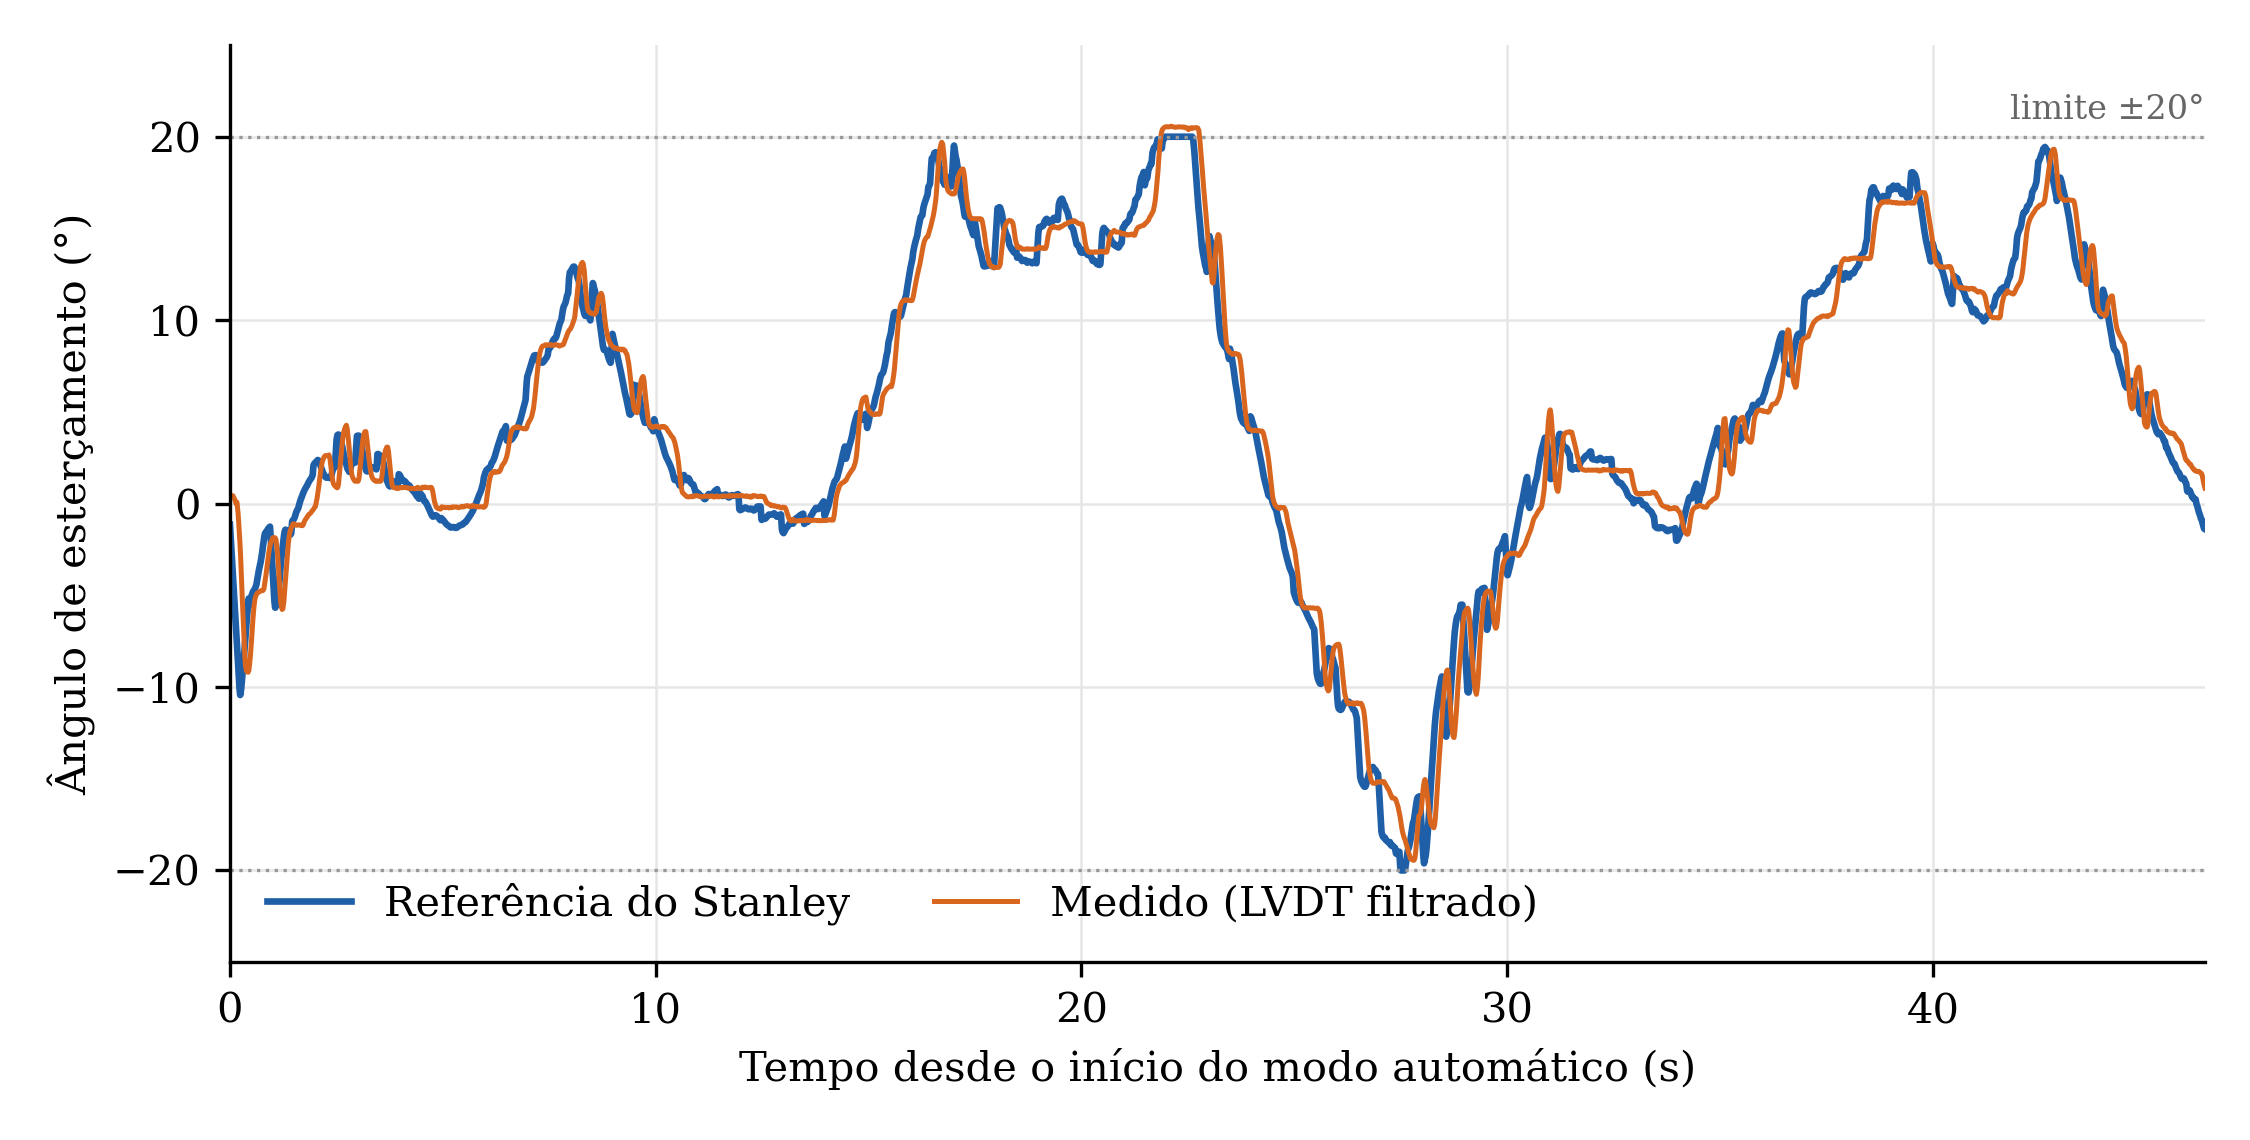
\includegraphics[width=\columnwidth]{Imagens/Resposta PID esterçamento.png}
    \caption{Resposta experimental do controlador de esterçamento. Fonte: Elaborado pelo autor.}
    \label{fig:resposta_esterçamento}
\end{figure}

Observa-se também que a resposta apresenta pequenos movimentos em degraus, especialmente durante variações reduzidas da referência. Esse comportamento resulta da interação entre a zona morta implementada no controlador, o atrito estático do mecanismo de direção e a ação integral. Enquanto o erro permanece dentro da zona morta, o acionamento é interrompido e o estado integral é mantido nulo.

Quando o erro excede esse limite e o atrito estático impede o movimento, a parcela integral aumenta progressivamente até que o esforço de controle seja suficiente para iniciar o deslocamento, que ocorre rapidamente até as proximidades da referência. Esse ciclo de adesão e deslizamento (\textit{stick-slip}) é característico de sistemas com atrito estático submetidos a controladores com ação integral. Como o estado integral é reinicializado na zona morta e ao cruzar a referência, além de ser limitado em amplitude, o esforço acumulado não se propaga entre ciclos consecutivos.

Por sua vez, o controlador PI de velocidade longitudinal foi avaliado quanto à capacidade de manter a velocidade do veículo próxima à referência de 2,0~m/s ao longo do seguimento autônomo de trajetória. Conforme apresentado na Figura~\ref{fig:resposta_velocidade}, a velocidade medida apresentou pequenas oscilações em torno da referência. Em regime permanente, a velocidade média foi de 1,998~m/s, com RMSE de 0,063~m/s, equivalente a aproximadamente 3,2\% da velocidade de referência. O erro máximo absoluto registrado foi de 0,187~m/s.

\begin{figure}[htb]
    \centering
    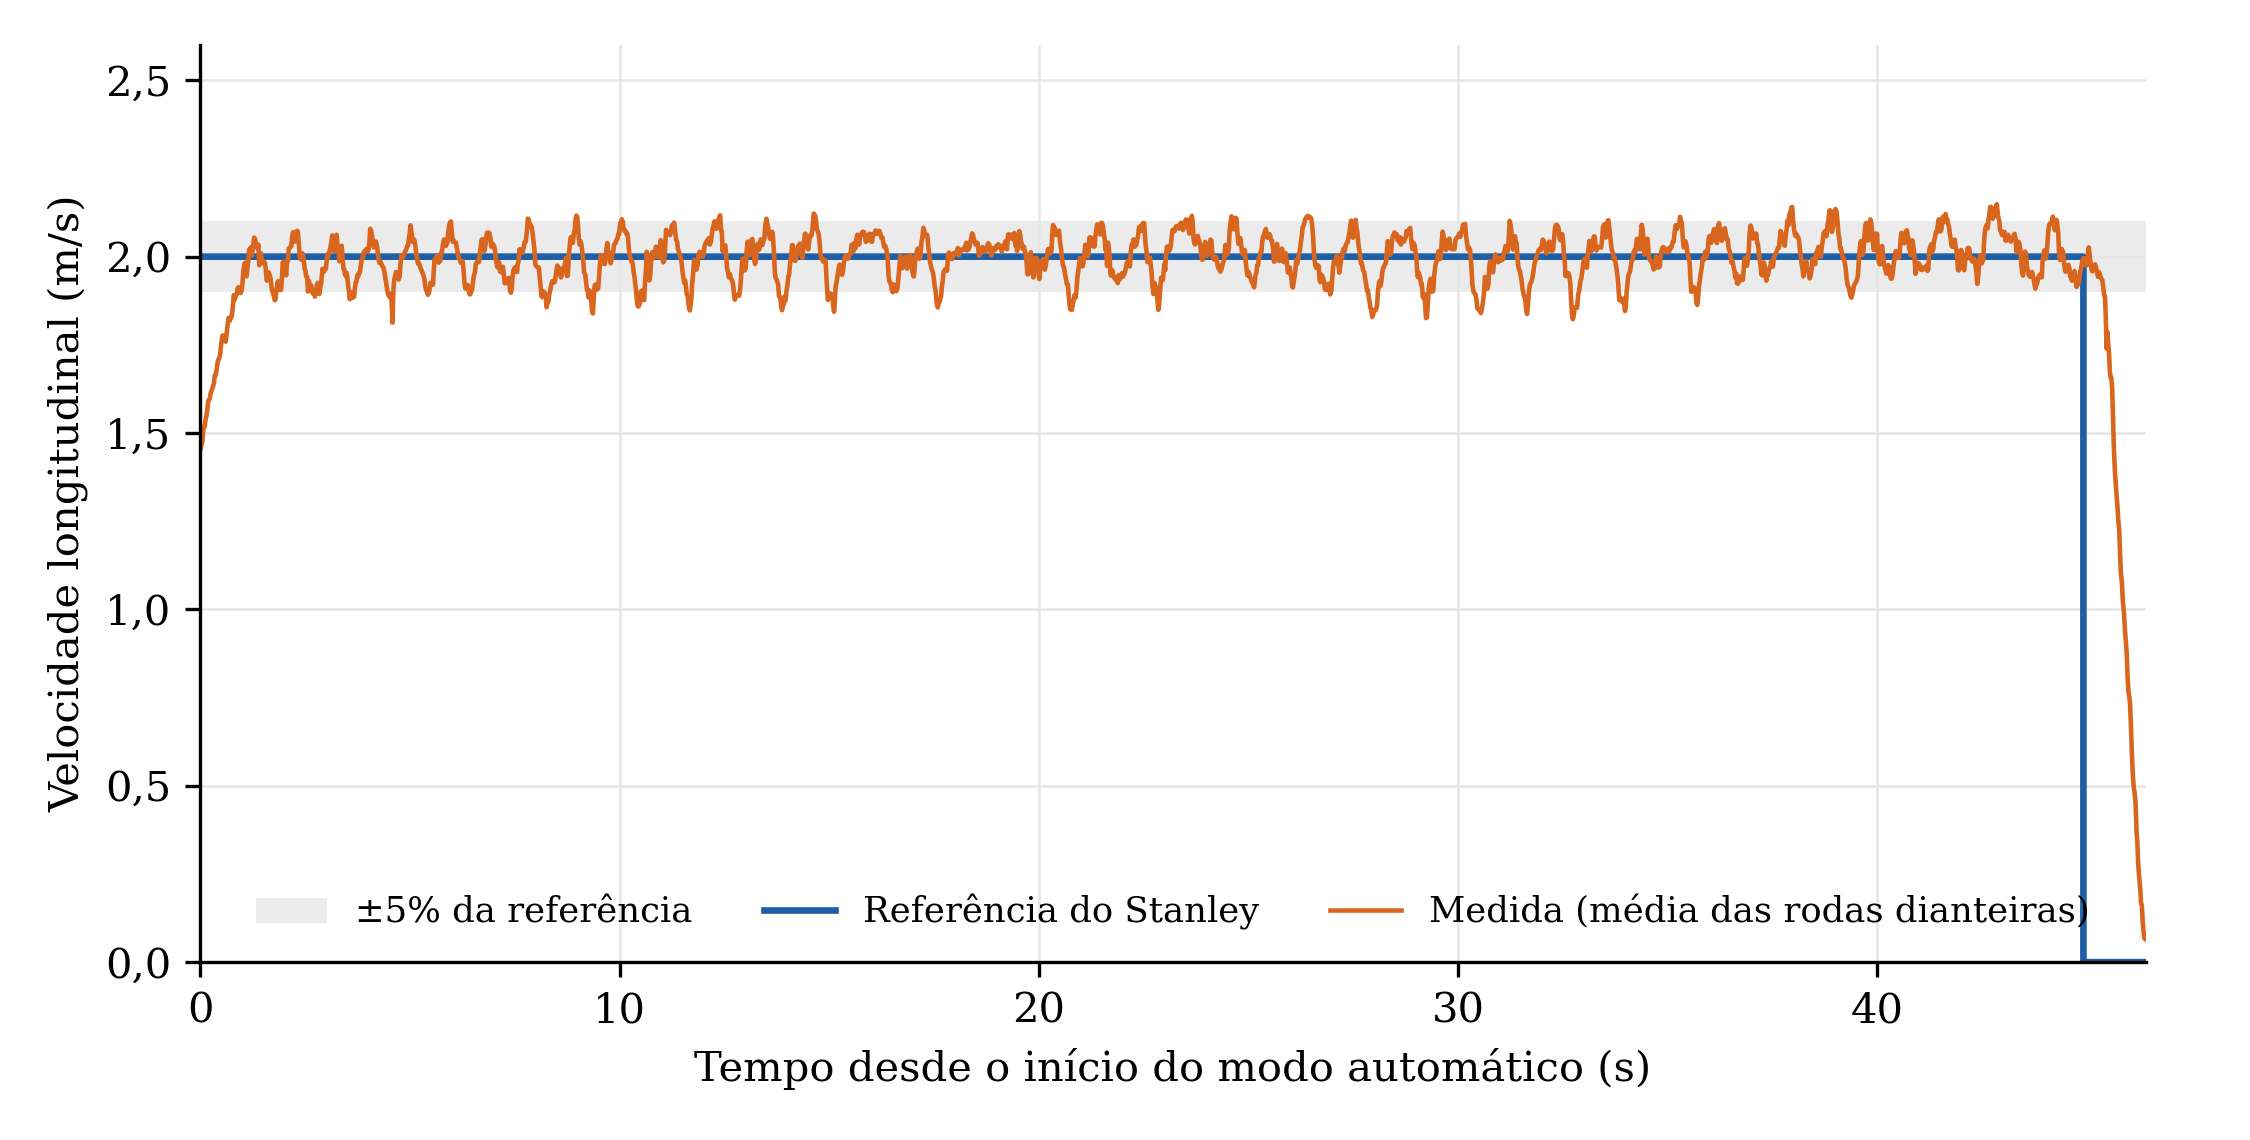
\includegraphics[width=\columnwidth]{Imagens/Resposta PI velocidadade longitudinal.png}
    \caption{Resposta experimental do controlador de velocidade longitudinal. Fonte: Elaborado pelo autor.}
    \label{fig:resposta_velocidade}
\end{figure}

As oscilações observadas estão relacionadas à zona morta de acionamento do motor, que exige um sinal PWM mínimo de aproximadamente 7,8\% para produzir o acionamento do módulo de conversão de potência. Entretanto, o acionamento médio necessário para manter a velocidade de referência corresponde a aproximadamente 7,5\% do PWM. Dessa forma, o menor acionamento disponível produz uma aceleração superior à necessária, fazendo com que a velocidade ultrapasse a referência. O controlador PI então interrompe a tração, permitindo que o veículo desacelere naturalmente devido às resistências ao movimento. Quando a velocidade retorna a valores inferiores à referência, a tração é restabelecida, produzindo oscilações periódicas em torno da velocidade desejada. A análise da saída do controlador confirma esse comportamento: em regime, o PWM de tração permaneceu entre 20 e 26, distante do limite de saturação de 50, e o freio não foi acionado. A parcela integral manteve-se aproximadamente constante, enquanto a oscilação do esforço de controle foi conduzida pela parcela proporcional, indicando que o fenômeno decorre da zona morta do acionamento, e não do acúmulo da ação integral. A Figura~\ref{fig:pwm_parcelas_pi_velocidade} apresenta o comportamento do PWM aplicado e das parcelas proporcional e integral do controlador em regime permanente.

\begin{figure}[htb]
    \centering
    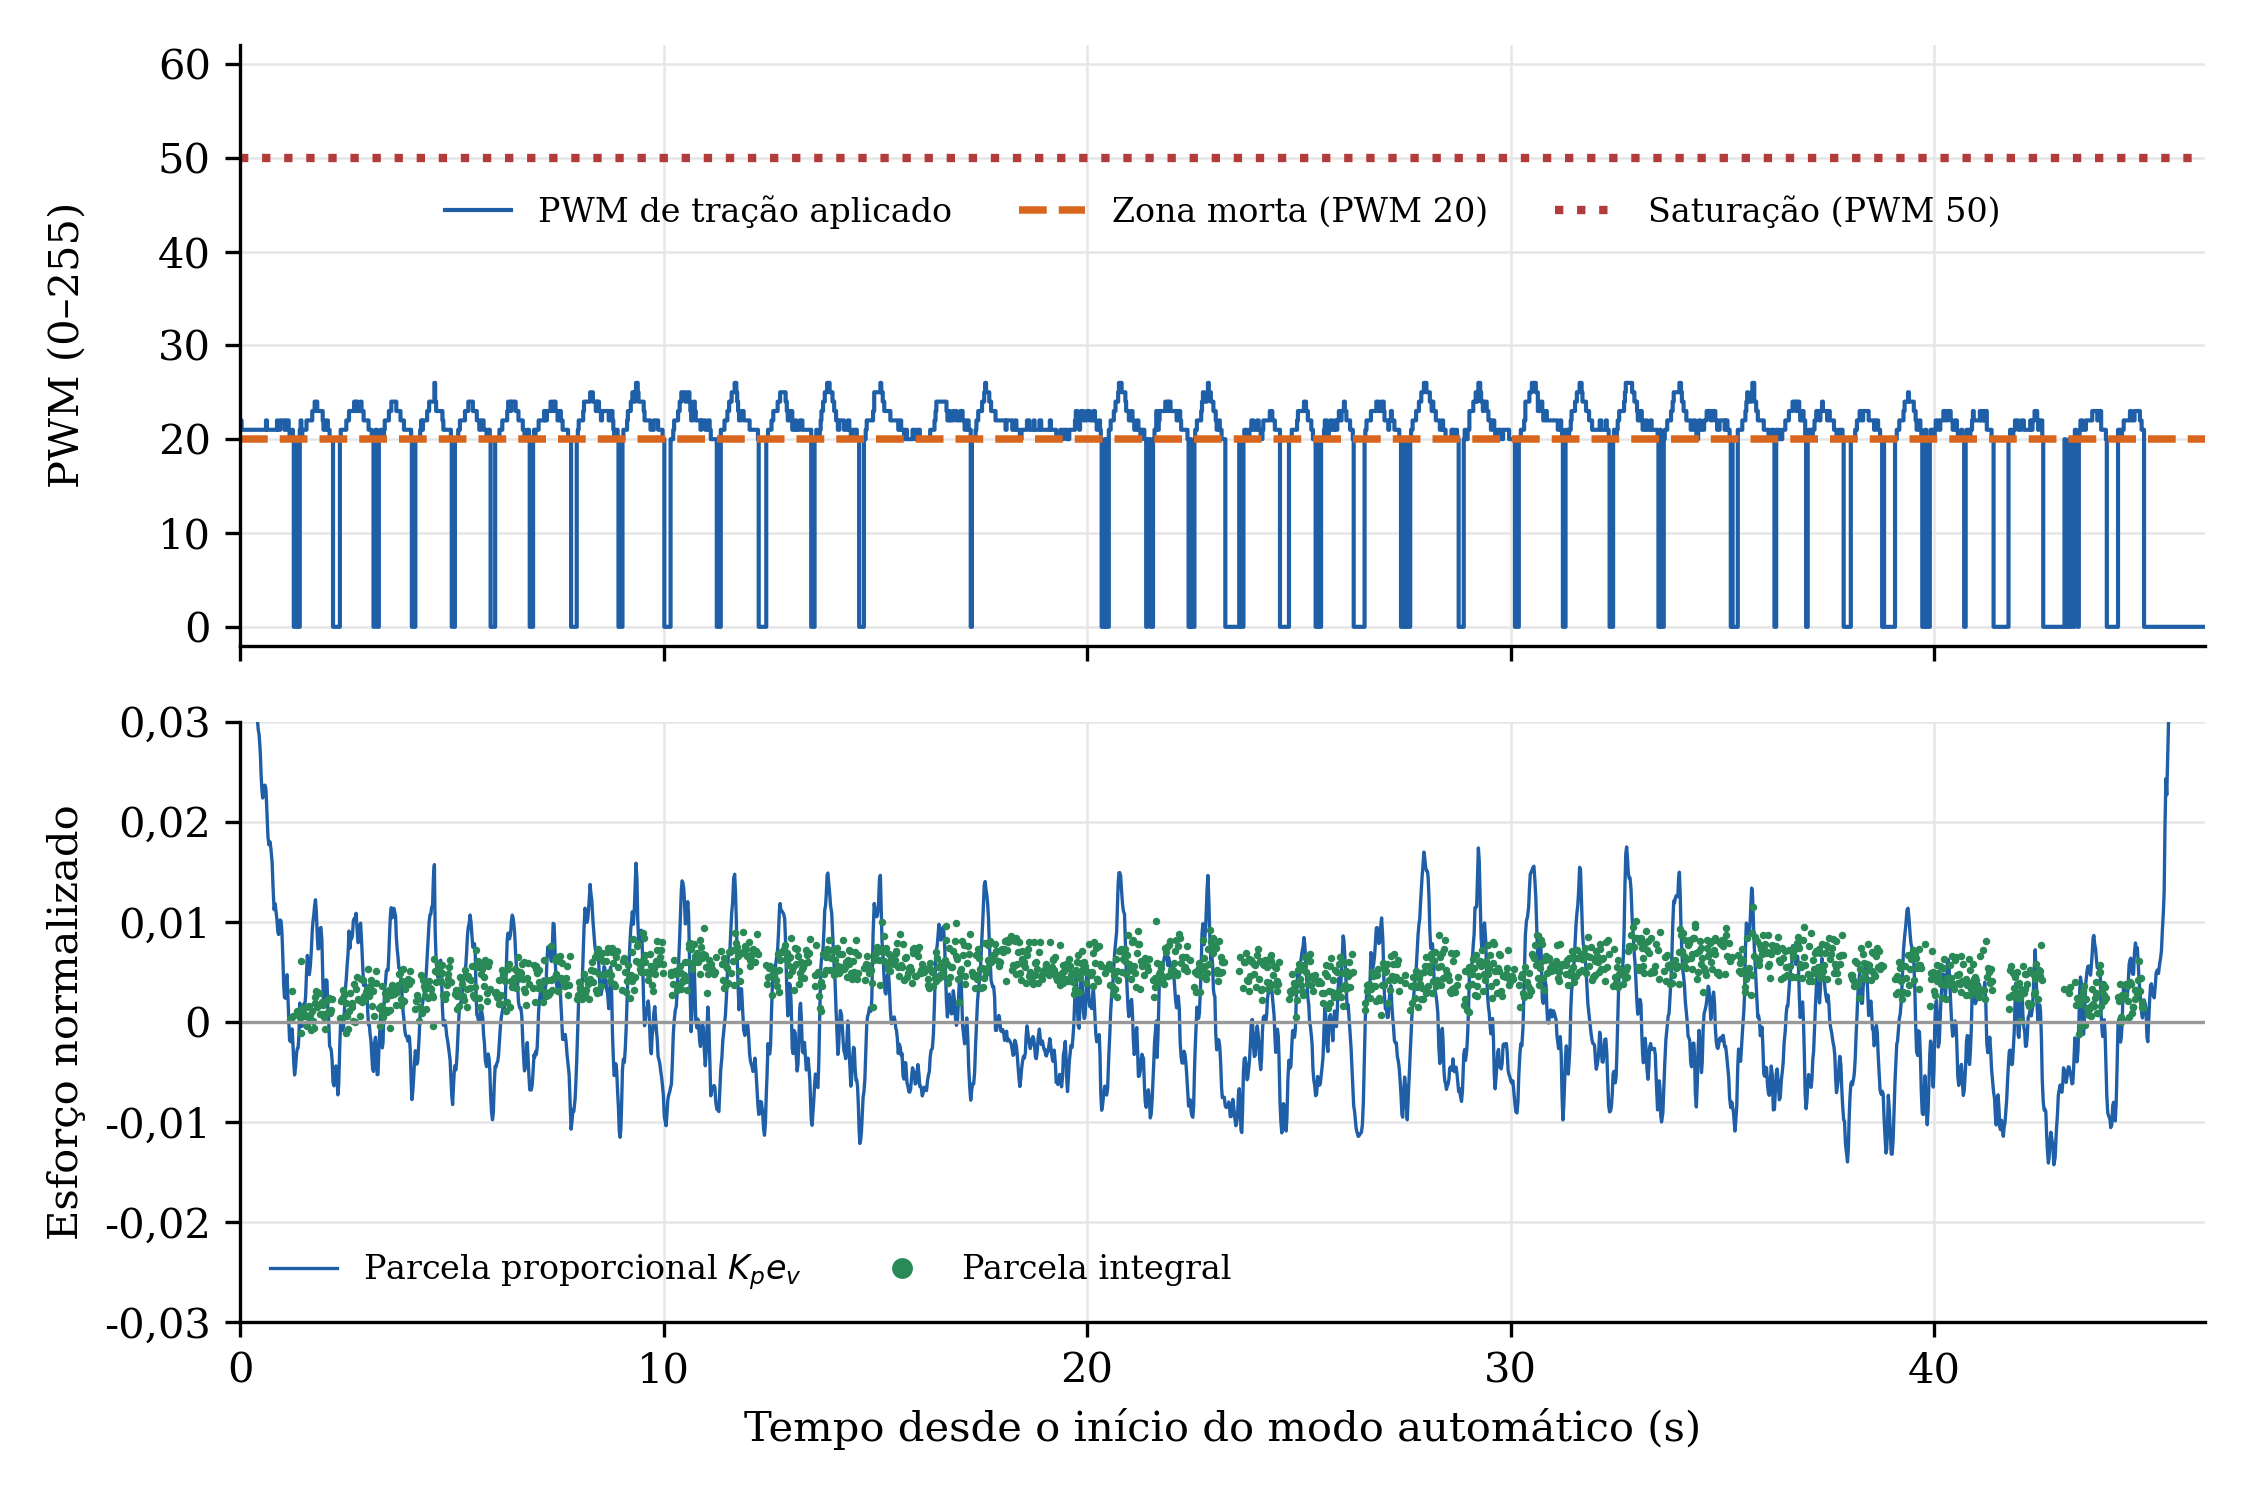
\includegraphics[width=\columnwidth]{Imagens/pwm_parcelas_pi_velocidade.png}
    \caption{Análise da saída do controlador PI de velocidade longitudinal e parcelas de controle. Fonte: Elaborado pelo autor.}
    \label{fig:pwm_parcelas_pi_velocidade}
\end{figure}

Apesar dessas oscilações, o controlador apresentou desempenho satisfatório na manutenção da velocidade longitudinal. Em regime permanente, o veículo permaneceu 88,6\% do tempo dentro de uma faixa de tolerância de $\pm 5\%$ em relação à referência e 100\% do tempo dentro de $\pm 10\%$. Esse comportamento é favorecido pela inércia do veículo, que suaviza as variações de velocidade provocadas pelos acionamentos intermitentes do motor de tração.


\subsection{Seguimento de Trajetória: Trajeto 1}

O primeiro ensaio de seguimento autônomo de trajetória foi realizado em um estacionamento localizado nas proximidades do Departamento de Engenharia de Alimentos da Universidade Federal de Lavras (UFLA). O local apresenta uma área aberta, favorável à recepção dos sinais GNSS e à realização dos experimentos com a plataforma VIDA.

No ensaio, o veículo percorreu aproximadamente 89~m em modo automático, ao longo de 46,5~s, mantendo velocidade média de 1,97~m/s, próxima à referência de 2,0~m/s. A Figura~\ref{fig:trajeto_1} apresenta a comparação entre a trajetória de referência e o percurso realizado pelo veículo.


\begin{figure}[htb]
    \centering
    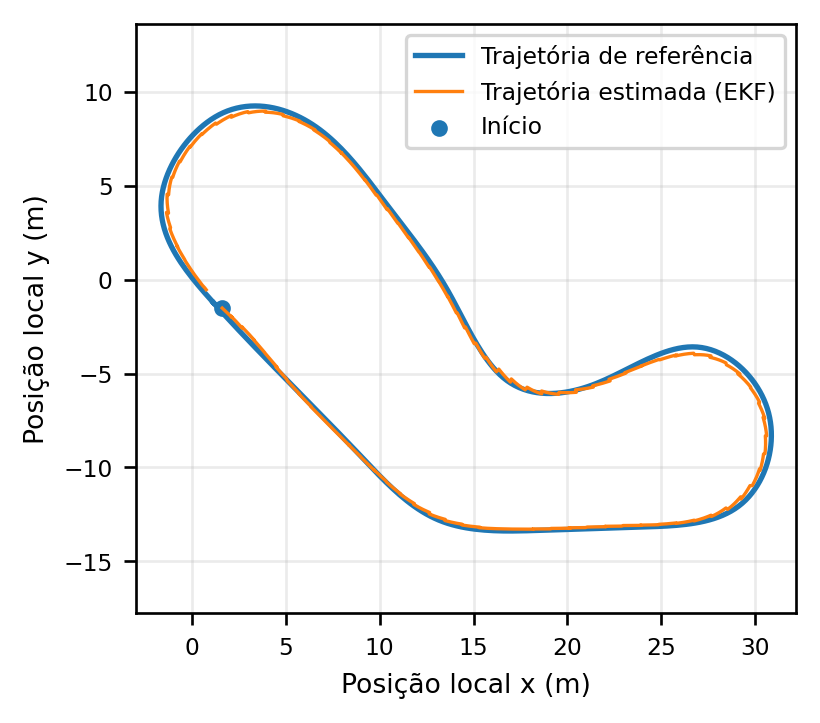
\includegraphics[width=\columnwidth]{Imagens/Trajetoria_Troia.png}
    \caption{Comparação entre a trajetória de referência e a trajetória percorrida pelo veículo no Trajeto 1. Fonte: Elaborado pelo autor.}
    \label{fig:trajeto_1}
\end{figure}

A avaliação do desempenho do controlador Stanley foi realizada a partir do erro lateral de seguimento. A Figura~\ref{fig:erro_lateral_trajeto_1} apresenta a evolução desse erro durante o percurso.

\begin{figure}[htb]
    \centering
    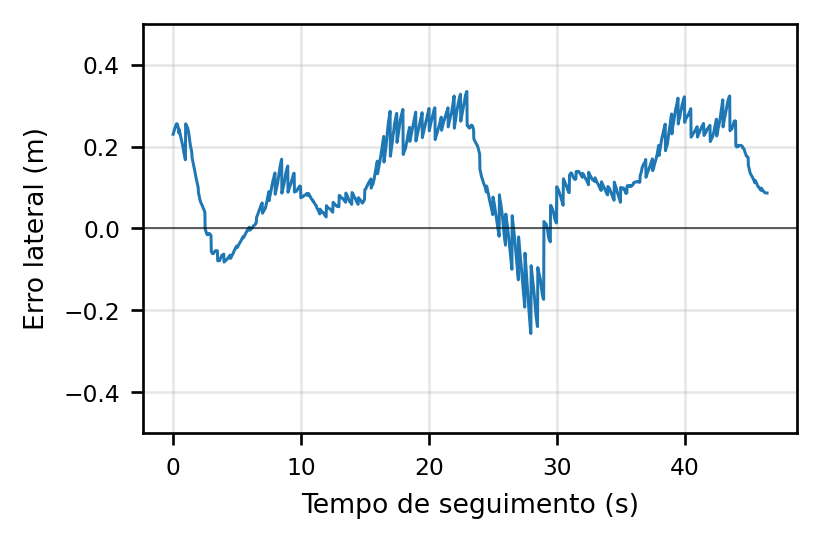
\includegraphics[width=0.85\columnwidth]{Imagens/Erro_Lateral_Troia.png}
    \caption{Evolução do erro lateral de seguimento durante o Trajeto 1. Fonte: Elaborado pelo autor.}
    \label{fig:erro_lateral_trajeto_1}
\end{figure}

O erro lateral apresentou raiz do erro quadrático médio (RMSE) de 0,167~m e valor máximo absoluto de 0,33~m. Observa-se também que o erro lateral apresenta, em alguns trechos, um padrão em dentes de serra, em vez de uma variação suave. Esse comportamento está associado ao processo de fusão de sensores do estimador de estados. Entre duas medições consecutivas do receptor GNSS, recebidas a 2~Hz, a posição do veículo é propagada pelo modelo de predição a partir da odometria, do ângulo de esterçamento e do giroscópio, acumulando um pequeno desvio que faz o erro lateral variar gradualmente. A cada nova medição GNSS, a etapa de correção reposiciona a estimativa, produzindo uma variação abrupta do erro. A análise dos registros confirma essa relação: o erro lateral apresenta uma componente periódica de 2~Hz, coincidente com a frequência de atualização do receptor GNSS, e as variações abruptas ocorrem, em média, cerca de 12~ms após a chegada de cada medição. Como essas variações ocorrem sempre no mesmo sentido, elas indicam um pequeno desvio sistemático do modelo de predição em relação às medições GNSS, possivelmente associado a erros de escala na velocidade medida ou de calibração do ângulo de esterçamento. 

Os resultados indicam que o controlador Stanley foi capaz de conduzir a plataforma VIDA ao longo da trajetória estabelecida, mantendo desvios laterais relativamente pequenos durante o percurso. Dessa forma, o ensaio demonstrou o funcionamento integrado dos subsistemas de localização, navegação e controle no seguimento automático de trajetória. A partir desse resultado, foi realizado um segundo ensaio em um percurso mais extenso, apresentado a seguir.



\subsection{Seguimento de Trajetória: Trajeto 2}
\label{subsec:trajeto_2}

O segundo ensaio de seguimento autônomo de trajetória foi realizado no autódromo da Universidade Federal de Lavras (UFLA), utilizando um percurso mais extenso e com diferentes características geométricas em relação ao primeiro experimento. A trajetória apresenta curvas e mudanças de direção, permitindo avaliar o desempenho do controlador Stanley em meio à execução de manobras sucessivas. Assim como no Trajeto 1, foram mantidos os parâmetros do controlador apresentados na Tabela~\ref{tab:parametros_stanley}, de modo que os dois ensaios fossem realizados sob a mesma configuração.

\begin{figure}[htb]
    \centering
    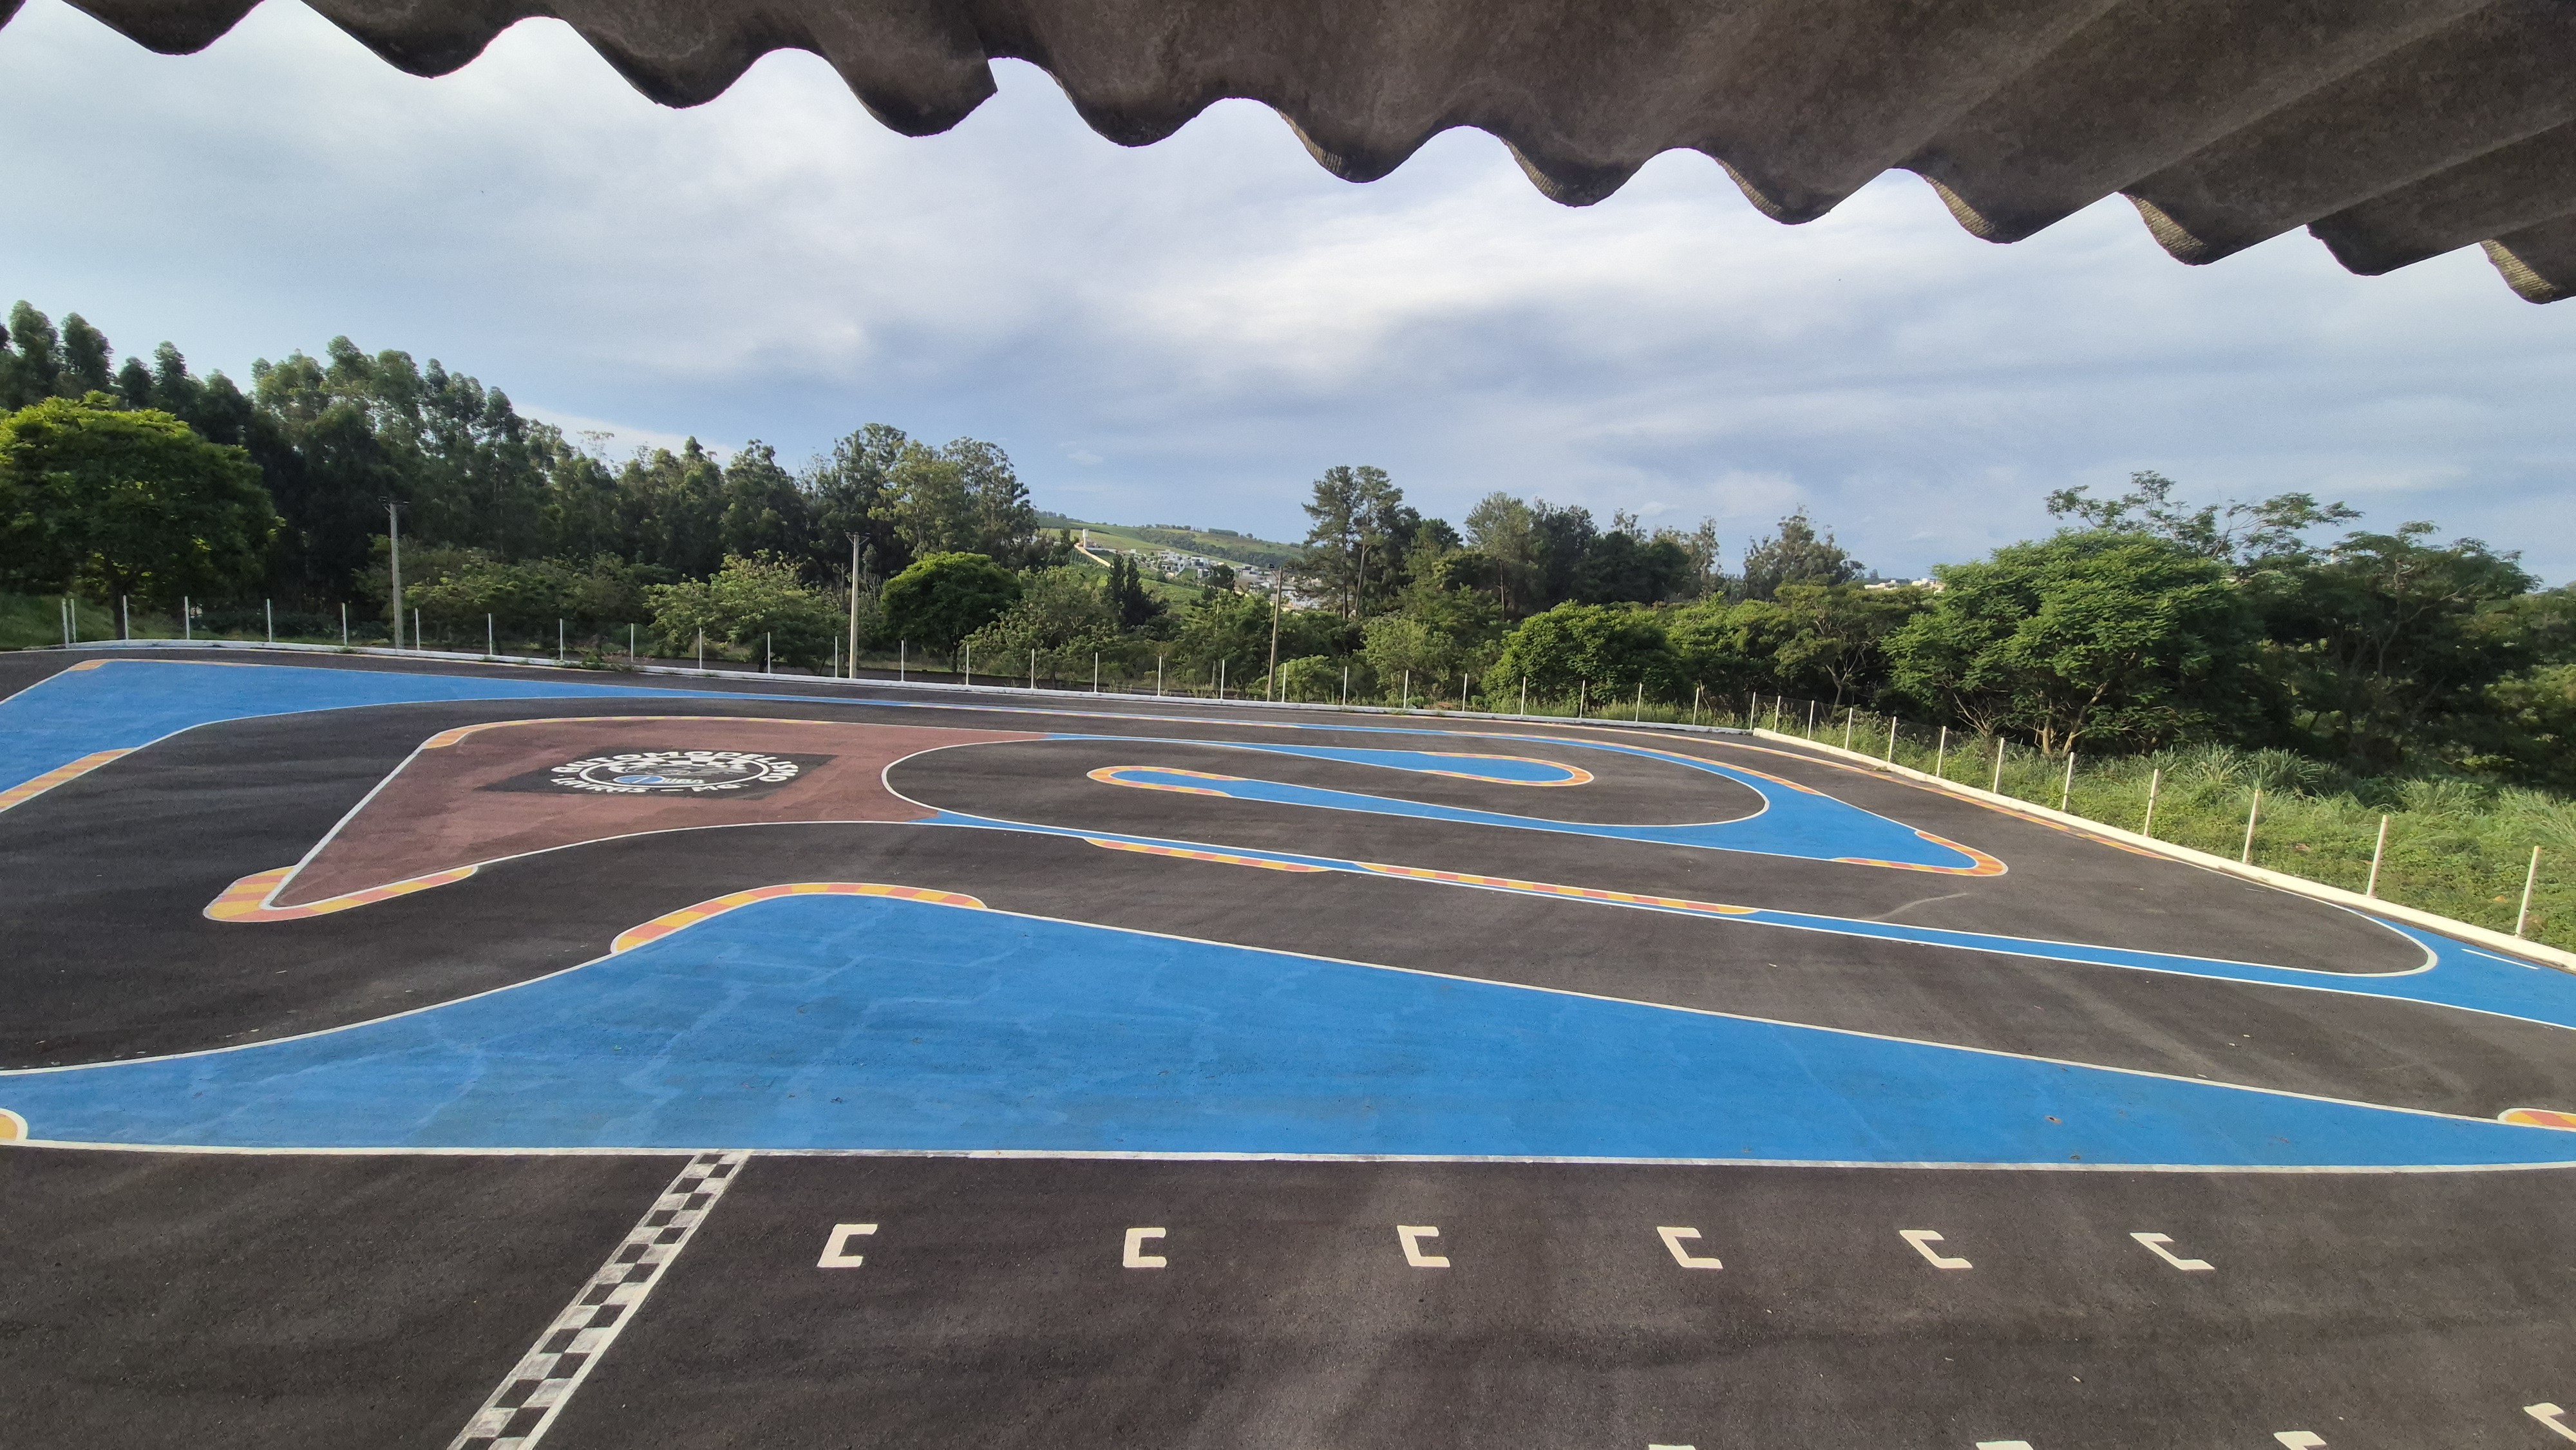
\includegraphics[width=\columnwidth]{Imagens/Autodromo_UFLA.jpg}
    \caption{Vista geral do autódromo da Universidade Federal de Lavras, utilizado no ensaio de seguimento autônomo de trajetória do Trajeto 2. Fonte: Acervo do autor.}
    \label{fig:pista_trajeto_2}
    
\end{figure}

O veículo percorreu de forma autônoma aproximadamente 281,42~m ao longo de 146,56~s, utilizando uma velocidade de referência de 2,0~m/s. A Figura~\ref{fig:trajeto_2} apresenta a comparação entre a trajetória de referência e o percurso realizado pelo veículo.

\begin{figure}[htb]
    \centering
    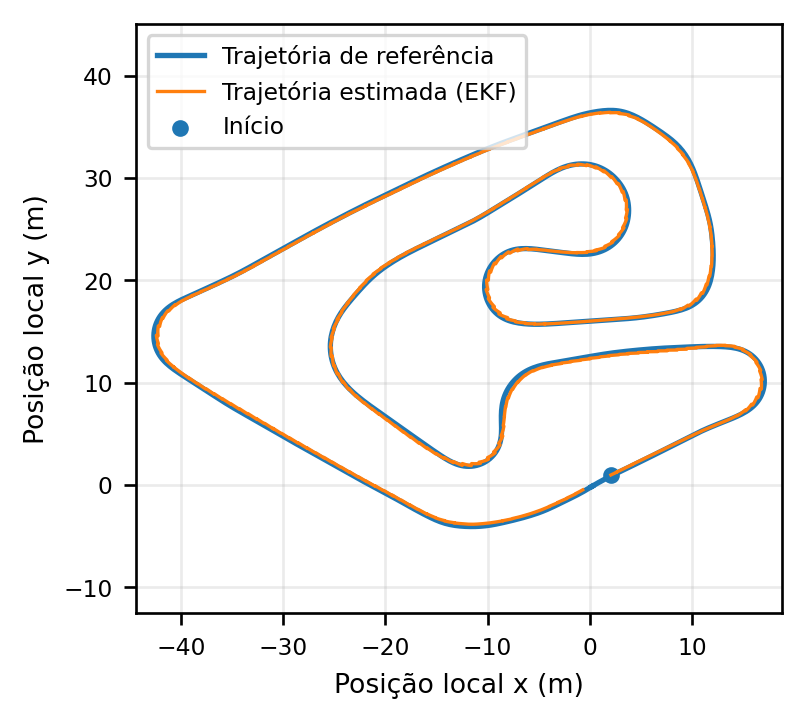
\includegraphics[width=\columnwidth]{Imagens/Trajetoria_Pista3.png}
    \caption{Comparação entre a trajetória de referência e a trajetória percorrida pelo veículo no Trajeto 2. Fonte: Elaborado pelo autor.}
    \label{fig:trajeto_2}
    
\end{figure}

Observa-se que o veículo foi capaz de acompanhar a trajetória estabelecida ao longo do percurso, realizando as correções de esterçamento necessárias para compensar os desvios laterais e de orientação. A execução desse experimento é particularmente relevante por envolver um trajeto mais extenso, exigindo a atuação contínua do controlador em diferentes condições de curvatura. A Figura~\ref{fig:erro_lateral_trajeto_2} apresenta a evolução temporal do erro lateral de seguimento durante o Trajeto 2.

\begin{figure}[htb]
    \centering
    \includegraphics[width=0.85\columnwidth]{Imagens/erro_lateral_Pista3.png}
    \caption{Evolução do erro lateral de seguimento durante o Trajeto 2. Fonte: Elaborado pelo autor.}
    \label{fig:erro_lateral_trajeto_2}
\end{figure}

Ao longo do experimento, o erro lateral médio absoluto (MAE) foi de 0,108~m, enquanto a raiz do erro quadrático médio (RMSE) apresentou valor de 0,129~m. O maior erro absoluto registrado foi de aproximadamente 0,366~m.

Esses resultados demonstram que o controlador Stanley foi capaz de manter o veículo próximo à trajetória de referência, mesmo diante das diferentes condições geométricas do percurso. Ao final do trajeto, o sistema de navegação identificou a conclusão da trajetória e realizou a transição para a condição de parada, evidenciando o funcionamento integrado dos sistemas de localização, navegação e controle da plataforma VIDA.

\subsection{Análise Comparativa dos Experimentos}

Os resultados quantitativos obtidos nos dois experimentos são apresentados na Tabela~\ref{tab:resultados_seguimento}. As métricas correspondem aos períodos de navegação autônoma identificados nos registros experimentais.

\begin{table}[htb]
    \centering
    \caption{Resultados experimentais do seguimento autônomo de trajetórias.}
    \label{tab:resultados_seguimento}
    \begin{tabular}{lcc}
        \hline
        \textbf{Métrica} & \textbf{Trajeto 1} & \textbf{Trajeto 2} \\
        \hline
        Percurso (m) & 89,24 & 281,42 \\
        Duração (s) & 46,48 & 146,56 \\
        MAE lateral (m) & 0,143 & 0,108 \\
        RMSE lateral (m) & 0,167 & 0,129 \\
        Erro máximo (m) & 0,334 & 0,366 \\
        Velocidade ref. (m/s) & 2,0 & 2,0 \\
        \hline
    \end{tabular}
\end{table}

A comparação demonstra que o sistema foi capaz de executar autonomamente dois percursos com diferentes comprimentos e características geométricas. O segundo experimento apresentou uma trajetória de referência com comprimento correspondente a aproximadamente 3,15 vezes o comprimento da primeira, mantendo valores reduzidos de erro lateral ao longo da execução.

No Trajeto 1, o RMSE lateral foi de 0,167~m, enquanto no Trajeto 2 foi de 0,129~m, representando uma redução aproximada de 22,8\% nessa métrica. De maneira semelhante, o MAE lateral diminuiu de 0,143~m para 0,108~m.

Entretanto, essa diferença não deve ser interpretada isoladamente como uma melhoria intrínseca do controlador, uma vez que os experimentos foram realizados em trajetórias distintas e podem apresentar diferenças de geometria, condições de superfície, alinhamento inicial e qualidade das estimativas de localização.

É importante destacar que as métricas de erro lateral foram calculadas a partir das estimativas utilizadas pelo próprio sistema de navegação. Dessa forma, representam o desempenho de seguimento avaliado no referencial do controlador, não constituindo uma medição independente da trajetória física efetivamente 
percorrida. Apesar dessa limitação, os experimentos representam uma validação funcional do sistema desenvolvido, demonstrando a capacidade de seguimento autônomo de trajetórias com valores de RMSE lateral inferiores a 0,17~m nas condições avaliadas.

\subsection{Validação da Arquitetura Computacional}
\label{subsec:validacao_arquitetura}

A análise dos registros de comunicação permitiu avaliar o comportamento da arquitetura computacional durante os experimentos, considerando os diferentes requisitos temporais de cada nível de processamento. No ESP32, as tarefas de aquisição, controle e segurança, executadas sob o FreeRTOS, operaram sem que fosse necessária a intervenção do supervisor de tarefas, responsável por bloquear o movimento caso alguma delas permaneça mais de 50~ms sem execução. Os tópicos publicados pelo ESP32 por meio do micro-ROS mantiveram entre 93\% e 95\% da frequência nominal de 50~Hz, com intervalos máximos de 40~ms entre mensagens.

Na Odroid e no notebook, os tópicos publicados pelos nós executados em ambiente Linux, com requisitos de tempo real flexível (\textit{soft real-time}), apresentaram frequências de publicação próximas à nominal de 50~Hz, com intervalos máximos de 27~ms, enquanto as medições GNSS foram recebidas regularmente a 2~Hz. Os intervalos observados nos tópicos de comando permaneceram inferiores ao limite de 200~ms adotado pelo ESP32 para identificar referências inválidas, indicando que as variações temporais não comprometeram a operação durante os ensaios.

A sequência de modos de operação, compreendendo as etapas de preparação, navegação autônoma e parada, também foi executada automaticamente, enquanto o painel de operação permitiu acompanhar os estados dos subsistemas e o progresso dos percursos. Esses resultados demonstram o funcionamento integrado dos três níveis de processamento e indicam que a distribuição das tarefas foi adequada às condições experimentais, concentrando as funções com requisitos temporais mais rigorosos no microcontrolador e distribuindo as demais entre a Odroid e o notebook.

De modo geral, os resultados demonstram que a integração do controlador Stanley, do sistema de estimação de estados e dos controladores de baixo nível possibilitou a execução autônoma das trajetórias avaliadas. Paralelamente, a análise do comportamento temporal e da comunicação entre os dispositivos evidenciou a viabilidade da arquitetura computacional distribuída nas condições experimentais. Dessa forma, o trabalho estabelece uma base funcional para futuros aprimoramentos dos sistemas de localização, controle, percepção e planejamento de trajetórias da plataforma VIDA.
